\documentclass{article}

\usepackage[utf8]{inputenc}
\usepackage{graphicx}
\usepackage{geometry}   \geometry{margin=1in}
\usepackage{amsmath}
\usepackage{xcolor}
\usepackage{float}
\usepackage{natbib}

\title{Hot Swappable Pedalboard and Routing System:\\Progress Report 1}
\author{Nicholas Pham}
\date{September 2018}

\begin{document}

\maketitle
\begin{center}
    Electrical Engineering \\
    Scott Kuindersma, Jim MacAurthur
\end{center}

\section{Overview}
	Many electric guitarists use effect pedals to augment their guitar amp's sound.  First developed in the 1960s, there are now thousands of pedals available for gutiarists to use.  Because of the plethora of options, guitarists need an easy way to compare and interchange effects.

	In my project proposal, I proposed an integrated \emph{hot-swappable} guitar effect pedalboard and switching unit to improve the efficiency by which guitarists can change out their effects pedals to create new sounds.  The proposal focused on two main use cases: performing musicians who need to quickly change sounds, and studio musicians who need ways to radically alter their sound via new combinations of effects.

	Through discussions with my advisors, the focus of this project has shifted away from the first use model to an expanded version of the second.  Following the first step of the design process \cite{ES100Lec3}, marketing, led to this shift of focus, as there are already products available that allow performing musicians to program combinations of effects to be switched on and off at once.  Now the product will aim less to be portable and usable in real-time by a gigging musician and more useful for off-line effects swapping.  As will be further described in the next section, the product will be designed as a sales tool for retailers such as Guitar Center who sell guitar effects pedals.  By making it easier for customers to try out new combinations of pedals, this product will help retailers sell more units, and help customers discover and purchase additional processors to expand and improve their guitar systems.

\section{Background and Existing Solutions}
	Though in an age of Internet shopping there are many guitar related products available for purchase on-line, most players want to test potential purchases in person before buying them.  As such, brick-and-mortar music stores such as Guitar Center still have a place in the industry.
	\subsection{Testing Effects}
	The existing method for testing effects pedals at brick-and-mortar retail store such as Guitar Center is a slow process.  Once a customer requests to test a pedal, an employee brings the particular unit being test to a padded table.  The employee must also find the correct power supply before connecting the unit to the guitar and the amplifier.  If a customer would like to test two pedals, for instance to decide between them which one to purchase, the employee would need to grab an additional power supply and cable for connection.  Then to perform an A-B test, the customer must turn the amplifier output off to prevent pops before disconnecting the current pedal and replacing it with the other one.  This time required for swapping the pedals limits the customer's ability to accurately judge the relative qualities of the units under test.  This cost can result in several negative consequences.  First, because of the reduction in accuracy of the A-B test, the guitarist may not be able to make a well-informed decision as to which effect best suits them, which could result in them either purchasing an inferior product, or in them deciding not to purchase any product at all.  Second, the known difficulties of testing effects pedals in this way may deter potential customers from even bothering at all, which limits the number of "impulse" purchases.  An improved method for testing guitar effects pedals at guitar stores would be beneficial to both consumers of these effects and their producers and retailers.

	\subsection{Sales Displays}
	While most of the in-stock effects pedals at retailers like Guitar Center are stored in a display for customers to peruse, some larger companies have integrated displays of their products.  For example, Figure \ref{fig:BossDisplay} shows one such display, containing products from Boss, one of the most popular companies in the industry \cite{ReverbMostPopular}.  As can be seen, the pedals are permanently attached to the display board, and are connected in series with power available to all effects at once.  This solves some of the issues mentioned previously.  For pedals that are available in these displays, employees do not need to do anything for customers to test them.  Customers must only plug a guitar into an input to the display unit, which automatically connects to the first pedal.  The last pedal in the series chain is always connected to a guitar amp.

	\begin{figure}
		\centering
		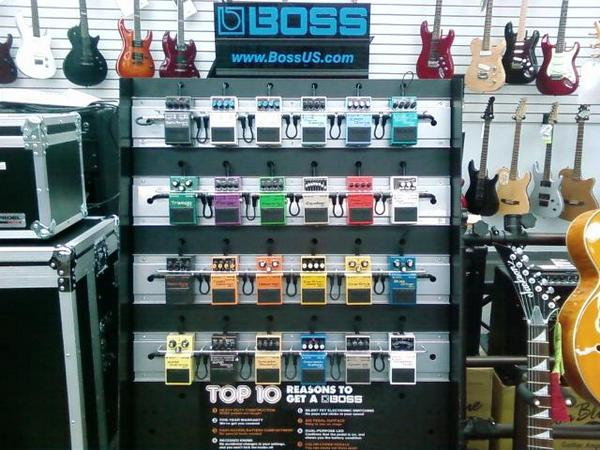
\includegraphics[width = 0.6 \textwidth]{BossDisplay.jpg}
		\caption{A display of Boss pedals typical to those found at retail stores such as Guitar Center \cite{BossDisplayPhoto}}
		\label{fig:BossDisplay}
	\end{figure}

	However, this system does have some limitations.  The first issue stems from the bypass method of many of these units.  Many guitar pedals, including all products offered by Boss, include a buffer that is active when the main "effect" is bypassed (see Figure \ref{fig:BufferedBypassConfig}).  This is useful for performing guitarists who often use cables totaling up to fifty feet in length.  The capacitive loading from the coaxial cable can result in high frequency loss, as guitar pickups can have DC output resistance on the order of $10k\Omega$.  A high input impedance and low output impedance buffer placed closer to the guitar can reduce the effects of this high frequency roll-off, which is typically undesirable.  However, because these display boards can contain up to thirty or more effects, there can be issues with signal degradation \cite{OrmanBypassMeasurements}.  This results in an inaccurate representation of the sound of any single pedal in the display.

	\begin{figure}
		\centering
		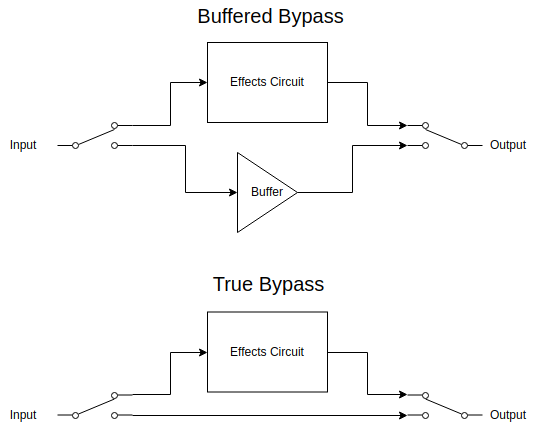
\includegraphics[width = 0.6 \textwidth]{BufferedvTrueBypass}
		\caption{Comparison of Buffered Bypass vs True Bypass topologies.  With the former, a buffer is in still placed in the signal even when the effect circuit is bypassed (some forms include the buffer prior to the effects circuit so the input is always buffered).  The true bypass topologies mechanically bypasses the effect circuit with a wire.}
		\label{fig:BufferedBypassConfig}
	\end{figure}


	Another issue is the fixed order and routing of the effects in the display.  The connection topologies between effects units can result in radical differences in output, which can affect the perceived quality of a pedals sound, when used in conjunction with others.  For example, consider the different topologies for connecting a distortion and delay pedal in Figure \ref{fig:PedalConnectionTopologies}.  The first one shows the guitar connected to the distortion pedal, which has its output connected to the input of a delay pedal, which in turn is connected to the guitar amplifier.  In this case, the sound might be the main distorted guitar sound with some dying echoes of the distorted sound.  The second topology shows the guitar connected to the distortion and delay pedals in parallel, which would result in the main distorted guitar sound and echoes of the "clean", unaffected guitar.  Finally, the third case shows the guitar first connected to the delay, which is them connected in series with the distortion pedal.  In this case, though the repeats of the delay decrease in amplitude over time, the non-linear clipping of the distortion pedal results in the echoes sounding at equal volume, all heavily distorted.  As can be seen even with this simple example involving only two effects, there are a multitude of possible connection topologies typically available to guitarists who own guitar pedals that are not available for testing on such display boards.

	\begin{figure}
		\centering
		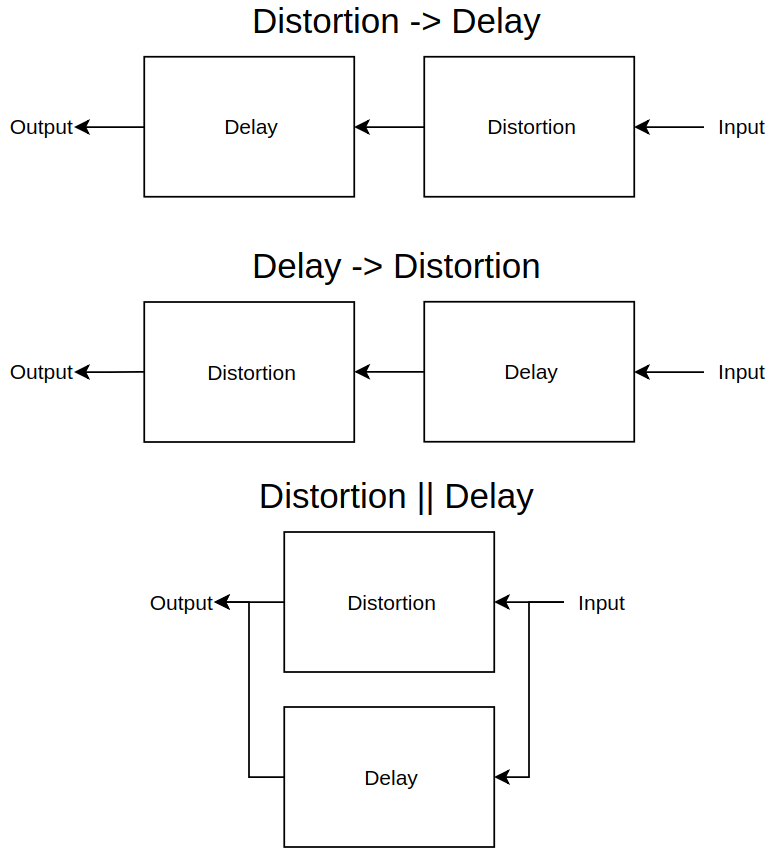
\includegraphics[width = 0.6 \textwidth]{RoutingConfigs.png}
		\caption{Example of the different ways to combine just two pedals.  More than two effects will have exponentially more options}
		\label{fig:PedalConnectionTopologies}
	\end{figure}

	\subsection{Studio Musicians}

	While this discussion has so far focused on guitarists as customers in a store, the same issues can face studio musicians hired for recordings.  These musicians must be able to produce any tone that their boss, the producer or artist who hired them, wants for the recording.  Because studio and musician time is very expensive, these studio musicians may have limited time to decide on and set up their equipment before recording begins.  Typically they might plug in pedals individually much as a customer does at a guitar store, which shares the issues described above.  Alternatively, some studio musicians might have their effects pedals integrated into an automatic switching system alluded to in the Overview.  However, these systems are often not intuitive to program, which means that the musician may set up a limited number of "presets", combinations of effects, that they will use.  This can limit their creativity in developing new sounds for their recordings.  A more intuitive system for connecting the effects pedals they already own would facilitate their creativity and save money by reducing the time spent on the mechanics of changing out equipment.

	\subsection{Prior Art}
	In addition to the displays mentioned above, there are several patents related to this project.

		\subsubsection{Magnetic Pedal Attachment}
		The Earthboard from Rare Earth Music LLC uses a unique system of magnets both to attach pedals to the pedalboard and to provide simple power to them.  Pedals are attached on a plate via a hook and loop device such as velcro.  Then the plates magnetically attach to long metal rails.  The two rails provide 9VDC power to the pedals via cabled connections between pedal and plate \cite{EARTHBOARDSITE}.

		\subsubsection{Bracket Attachment}

		U.S. Patent Grant US9620094B2 describes an improved method for attaching pedals to a pedalboard \cite{ABBATE:2016}.  Using small brackets which are directly mounted to the pedal enclosure via the bottom cover screws, this method for mounting pedals is much more stable and solid than velcro or zip-tie methods, while also using few external materials. However, this implementation describes directly attaching the pedals to the pedalboard, which will require other screws. This means the pedal placement will be fairly permanent and it will be difficult to swap out pedals, necessitating the use of external tools such as a screwdriver.

		\subsubsection{Modular Effect System}

		U.S. Patent US4479238A describes an effect system incorporating a main parent enclosure which contains power and signal routing circuits and receiving slots for effect modules \cite{SPECTOR:1982}. These modules contain effects circuits built into a special form factor that allows them to be inserted into the slots and make signal and power connections with the main unit. The main enclosure contains routing circuits which can choose, remotely or on the front panel, which effects should be connected, much like the automatic routing systems described previously. In addition, the housing automatically bypasses any slot in which no module is fully inserted, preventing issues with ”hot-swapping”, or removing the effect card while the system is in use. This system does a nice job of allowing different combinations of effects to be tested, but it does have a significant limitation. The effect modules must be of the correct card format, which limits the user to specifically designed units. As the guitar pedal form factor is so ubiquitous (though not exactly standardized: pedals may come in many shapes and sizes), a guitarist using this system would not be able to incorporate the majority of effects units offered today, and would not be able to use any pedals they already own. In addition, because of their design, these card modules cannot be used in absence of the main enclosure unlike normal guitar pedals, further limiting their flexibility.

		\subsubsection{Waterproof Swappable Effects System}

		U.S. Patent USD782567S1 describes a pedalboard system which allows guitar effects pedals to be attached magnetically to a pedalboard \cite{FAORO:2015board}.  The system allows for hot-swappability of effects, which are connected to the board's internal routing via contacts underneath: no external cables are required.  While the patent has very little detail on the capabilities and specifications of the product, it is available for sale from Nexi Industries \cite{NexiIndustries}.  Their website claims that the switching in both the pedals and on the board is "true bypass", which in industry terminology means that the effects circuits are mechanically switched out of the signal path when bypassed, as opposed to electronic switching with buffers mentioned above.  The initial system was designed to be used specifically with proprietary effects pedals, covered in U.S. Patent USD782566S1 \cite{FAORO:2015pedal}.  However, the manufacturer has since released a product to interface with third-party guitar effects \cite{conNEXI}.

		The product does offer a solution to many issues thus far described.  In particular, it allows for fast swapping of effects pedals without the need for unplugging signal and power cables.  However, it does have some issues.  The interface between the pedal and the plate still relies on uncontrolled lengths of cable required to make connections with the pedal's input and output jacks.  The system also supposes a single power supply type, 9VDC through a 2.1mm center negative plug.  While this is fairly standard, there are a number of popular effects, particularly more powerful digital ones, that require different power supplies.  There is also no improvement on the mechanism for attaching third party effects to the plates: the marketing examples show zip-ties being used, which can damage the pedal \cite{conNEXI}.  The pedal plates also only come in one size which is not suitable for many larger pedals.  Finally, the system supports only a single series routing option, which eliminates many possible routing topologies.

\section{System Diagram}
	\subsection{Overview}
	The architecture of the project roughly follows its physical form.  This is to ensure that the product is as user friendly and intuitive as possible.  Figure \ref{fig:OverviewScheme} shows the general structure.  The pedal plates are arranged in a grid.  Each row is typically connected in series, but there are switches in between each column to allow signal transfer between rows.  Figures \ref{fig:Series} and \ref{fig:Parallel} show two of the many possible routing configurations available.

	\begin{figure}
		\centering
		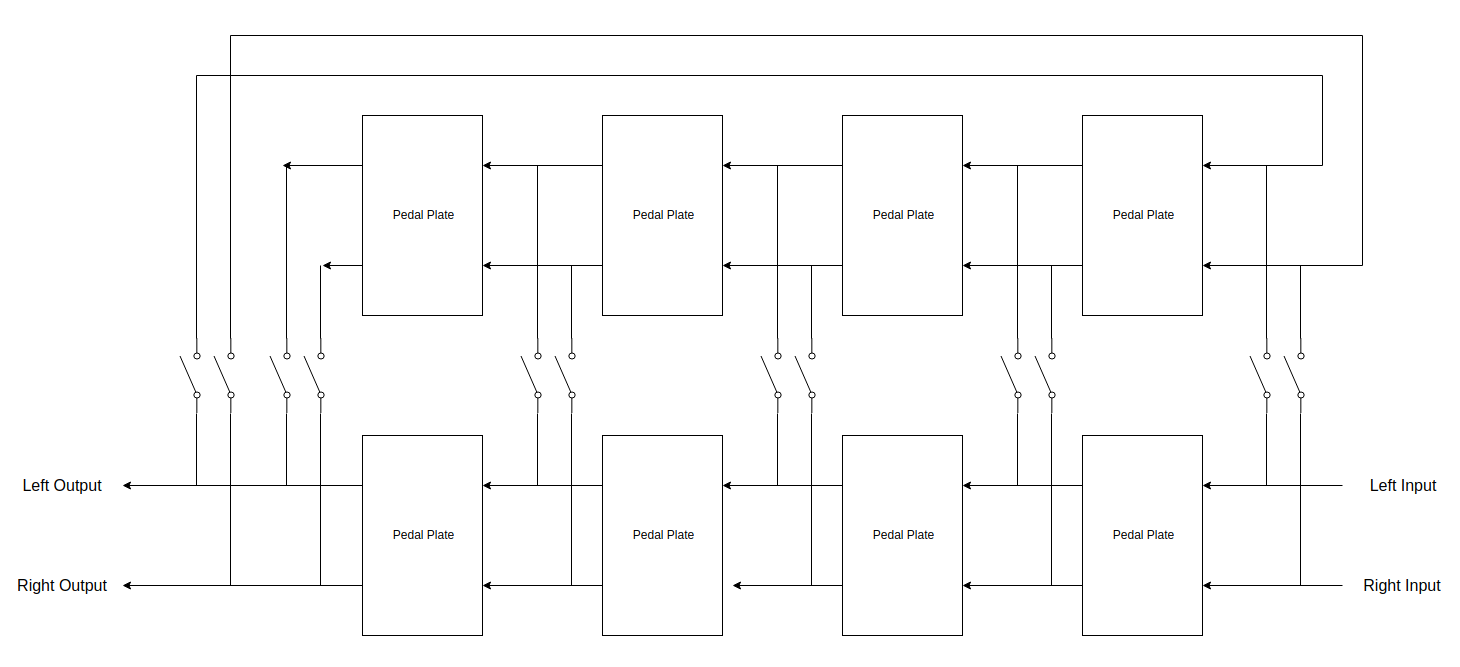
\includegraphics[width = \textwidth]{ES100PR1_OverviewScheme.png}
		\caption{Overview of Design Architecture.}
		\label{fig:OverviewScheme}
	\end{figure}

	Though this architecture limits the number of routing configurations from that described in the project proposal (any input could be routed into any output), there are still numerous options available.  This limitation resulted from two main considerations.  One is the user experience and interface, which is one of the most important and difficult design challenges that faces this project.  The improvement this product will make over existing automated switching systems is in user friendliness and intuitiveness.  Just as the user can intuitively move and replace pedals on the board, they should also be able to easily change the connection topology between series and parallel.  There is no need for a user to electronically swap the order any two pedals are in when connected in series, as they could physically switch their positions.  Therefore, the routing control needs only to concern parallel and series combinations.  The simplest way to accomplish this are switches that can be opened to connect the signals between rows, with some sort of mixing device if necessary.

	While the physical manifestation of the electrical connections poses a fairly small issue, the biggest design issue is the user interface for selecting different routings.  When the effects are all connected in series, the order of effects is visually obvious to users, but when using some parallel combinations such as that shown in Figure \ref{fig:Parallel}, this may not be obvious.  One solution is a system of visual cues: namely lights that would indicate the connections currently being made.  To interact with these, the lights may incorporate switches, which would provide a tactile and intuitive interface.  Such consideration will be tested on the second prototype (see Revised Schedule).

	\begin{figure}
		\centering
		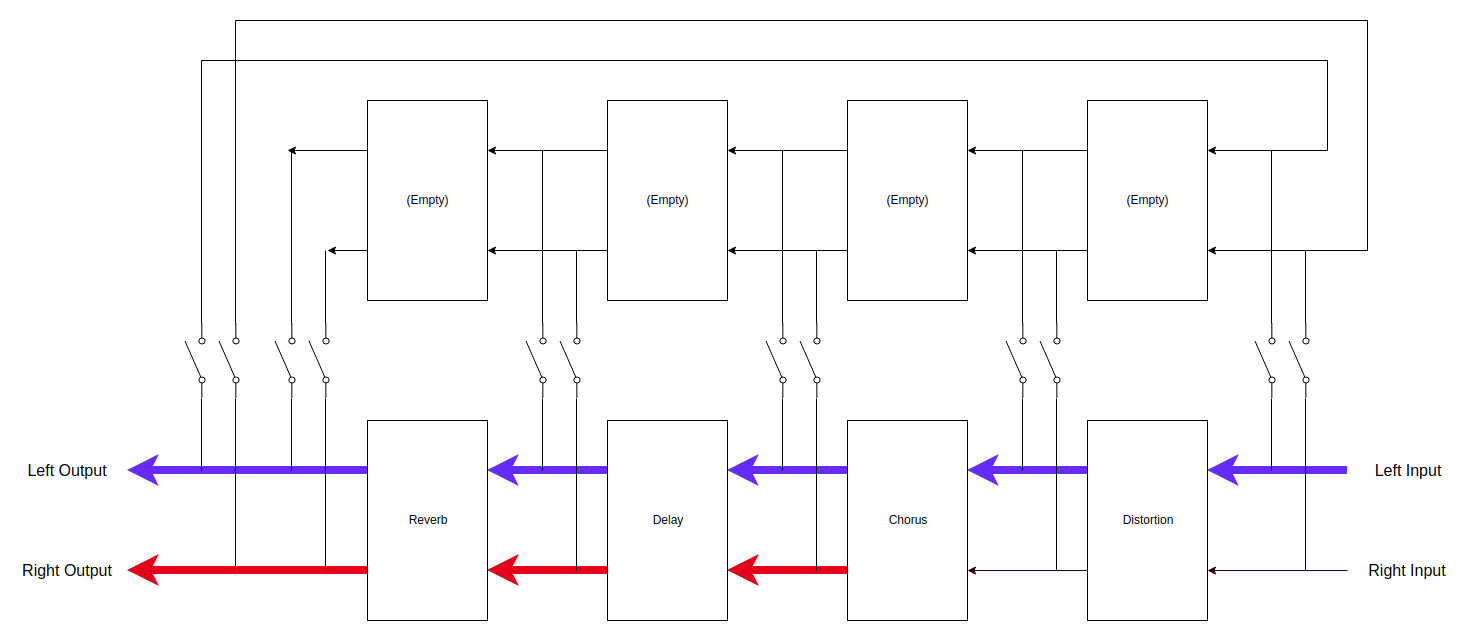
\includegraphics[width = \textwidth]{StereoSeriesRouting.png}
		\caption{Example of the general architecture set for a series routing topology, which includes both mono and stereo pedals.}
		\label{fig:Series}
	\end{figure}

	\begin{figure}
		\centering
		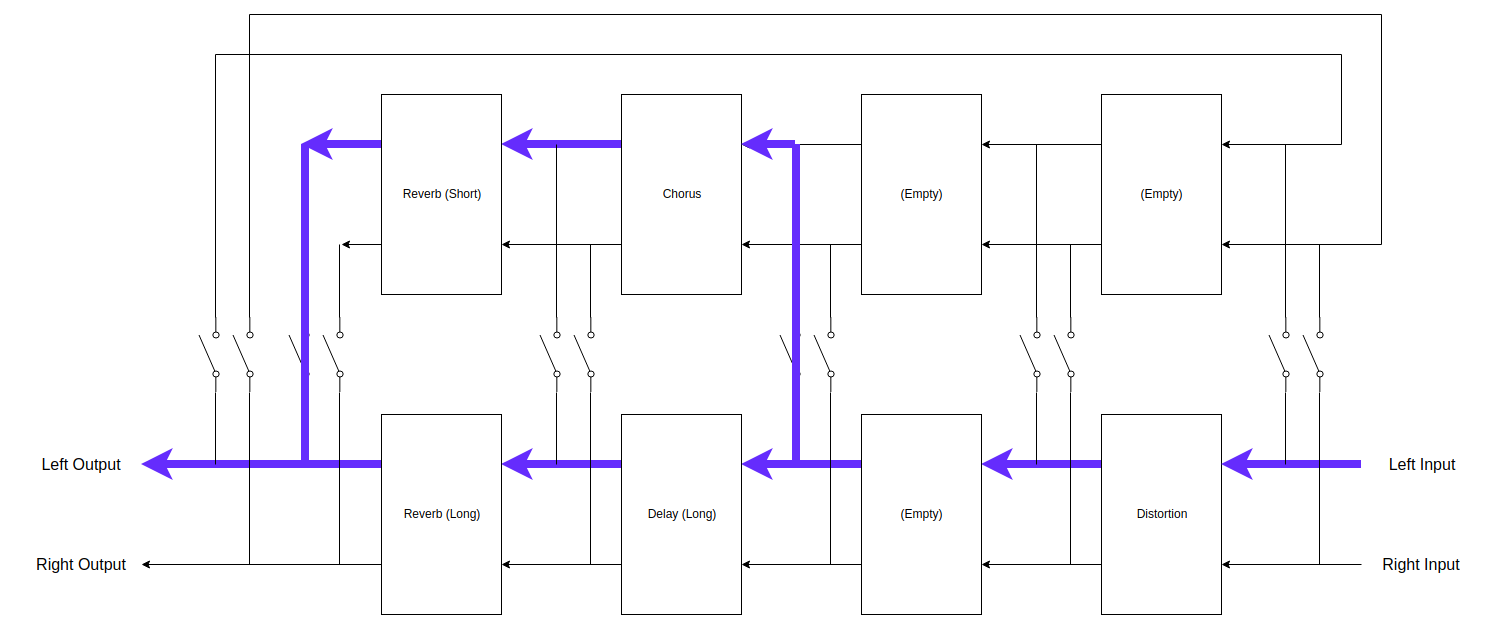
\includegraphics[width = \textwidth]{MonoParallelRouting.png}
		\caption{Example of the general architecture set for one possible topology involving a combination of series and parallel connections.}
		\label{fig:Parallel}
	\end{figure}

	\subsection{Pedal Mounting Techniques}
		\subsubsection{Through Screws}
		One important subsystem is the mounting of the pedals on their plates.  One attractive option is the use of screws through the pedal's bottom cover, as described in \cite{ABBATE:2016}.  This is the most visually simple technique, but relies on pedals that have similar screw hole locations.  As discussed below, while pedals from a single manufacturer tend to come in only a handful of form factors, the locations are not always standard across manufacturers.  In addition, some pedals do not have screws on opposite corners, which is required for a secure connection.  For instance, the Ibanez TS-9 Tubescreamer has bottom cover screws only on the upper (north) side of the pedal.  Because of this type of issue, the screw-through-plate method may not work for all pedals.

		\subsubsection{Clamp}
		Another option for attaching pedals to their plates is via a clamping mechanism.  Figure \ref{fig:CornerClamp} shows a preliminary design for such a clamp, which would be used to attach pedals with irregular bottom screws.  The bracket would be located in x-y position by the bolt hole to the corner of the pedal, and would be firmly held down in the z direction by a bolt clamping through the plate. The inner sides of the bracket should be rubber or a similar surface that will not damage the finish of the pedal.  Also see Figure \ref{fig:PedalPlateSubsystem} for an example of these brackets being used with a pedal.

		\begin{figure}
			\centering
			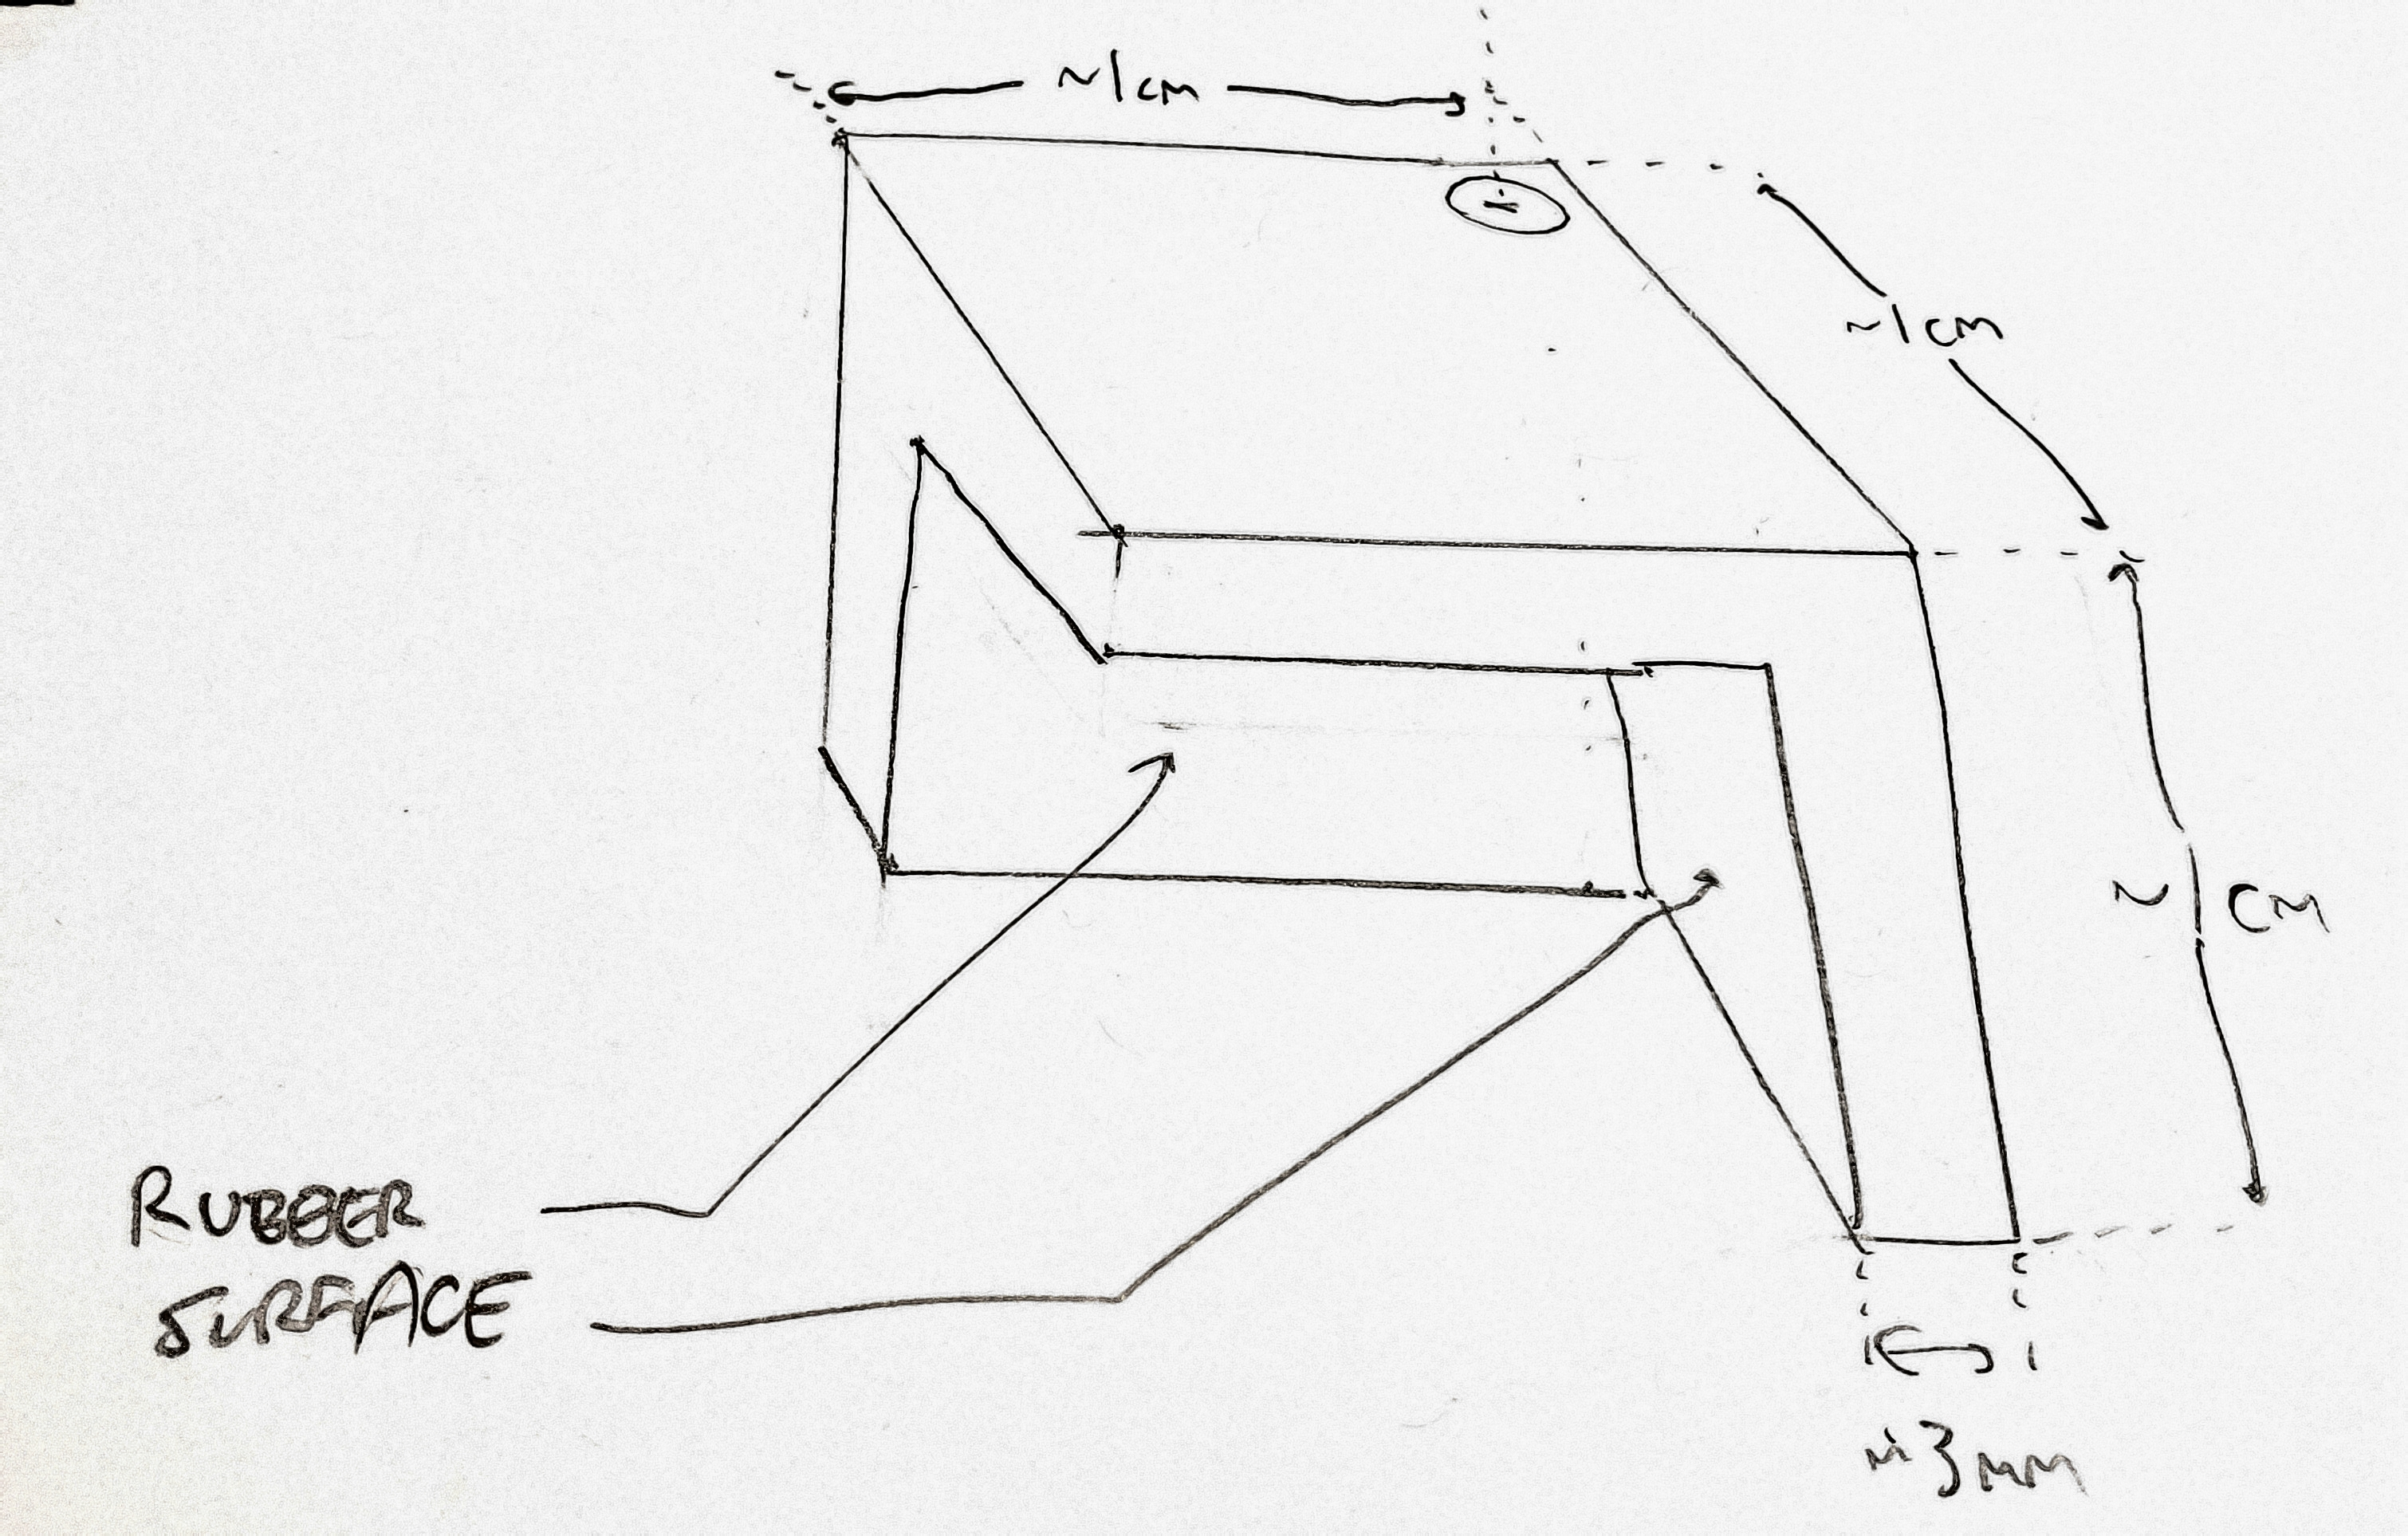
\includegraphics[width = 0.6 \textwidth]{CornerBracketPerspective.jpg}
			\caption{View of prospective design for corner clamp.}
			\label{fig:CornerClamp}
		\end{figure}

		\subsubsection{Linear Travel}
		Because of the incongruities between effects pedals of different manufactures, a single set of bolt holes through the pedal plate will not suffice to accommodate most effects.  To solve this, the design will incorporate some combination of multiple holes in different locations and some slots through which the bolts can pass.  The specific orientation of these holes and slots must be determined in some rapid prototyping prior to the fabrication of the first main prototype.  They should be judged according to their flexibility in accommodating effects pedals of various forms.

		\subsubsection{Electrical Connections}
		In addition to the solid mechanical connection between the guitar pedal and its mounting plate, there also needs to be electrical connections.  The pedal's native jacks should be used so as to not require modification of the unit for sale.  This requires a method for allowing plugs to be inserted into these jacks.  This poses and issue because of the irregularities in input, output, and power jack locations between companies, or even between pedals manufactured by the same company.  Although the signal input and output jacks are all 1/4" phone jacks, their location and number can vary significantly.  They can be located on the sides or on the top of the enclosure.  There can be multiple input and output jacks for stereo connections, as well as additional ones for external control devices, such as expression pedals.  A simple method for implementing these connection is a cable connected to each plug long enough to work on all possible pedals, such as the adapter unit sold with the aforementioned Nexi Industries pedalboard \cite{conNEXI}.  However, this is not ideal because the extra cable length can take up extra space, and when the cable is bent at sharp angles can leave it prone to damage after repetitive use.  A difficult design decision that must be made is the mechanism for connecting to the pedals with the least amount of excess cabling.  One option is some sort of retractable cable, similar to retractable ID badge reels.  The retractor could be placed on the plane of the plate and the orifice for the cable to escape might be on some turret above the plate to minimize sharp bends in the cable.  This is another design feature that must be rapid prototyped during ideation to find a workable solution.  See Figure \ref{fig:PedalPlateSubsystem} for a diagram of this integrated subsystem.

		\begin{figure}
			\centering
			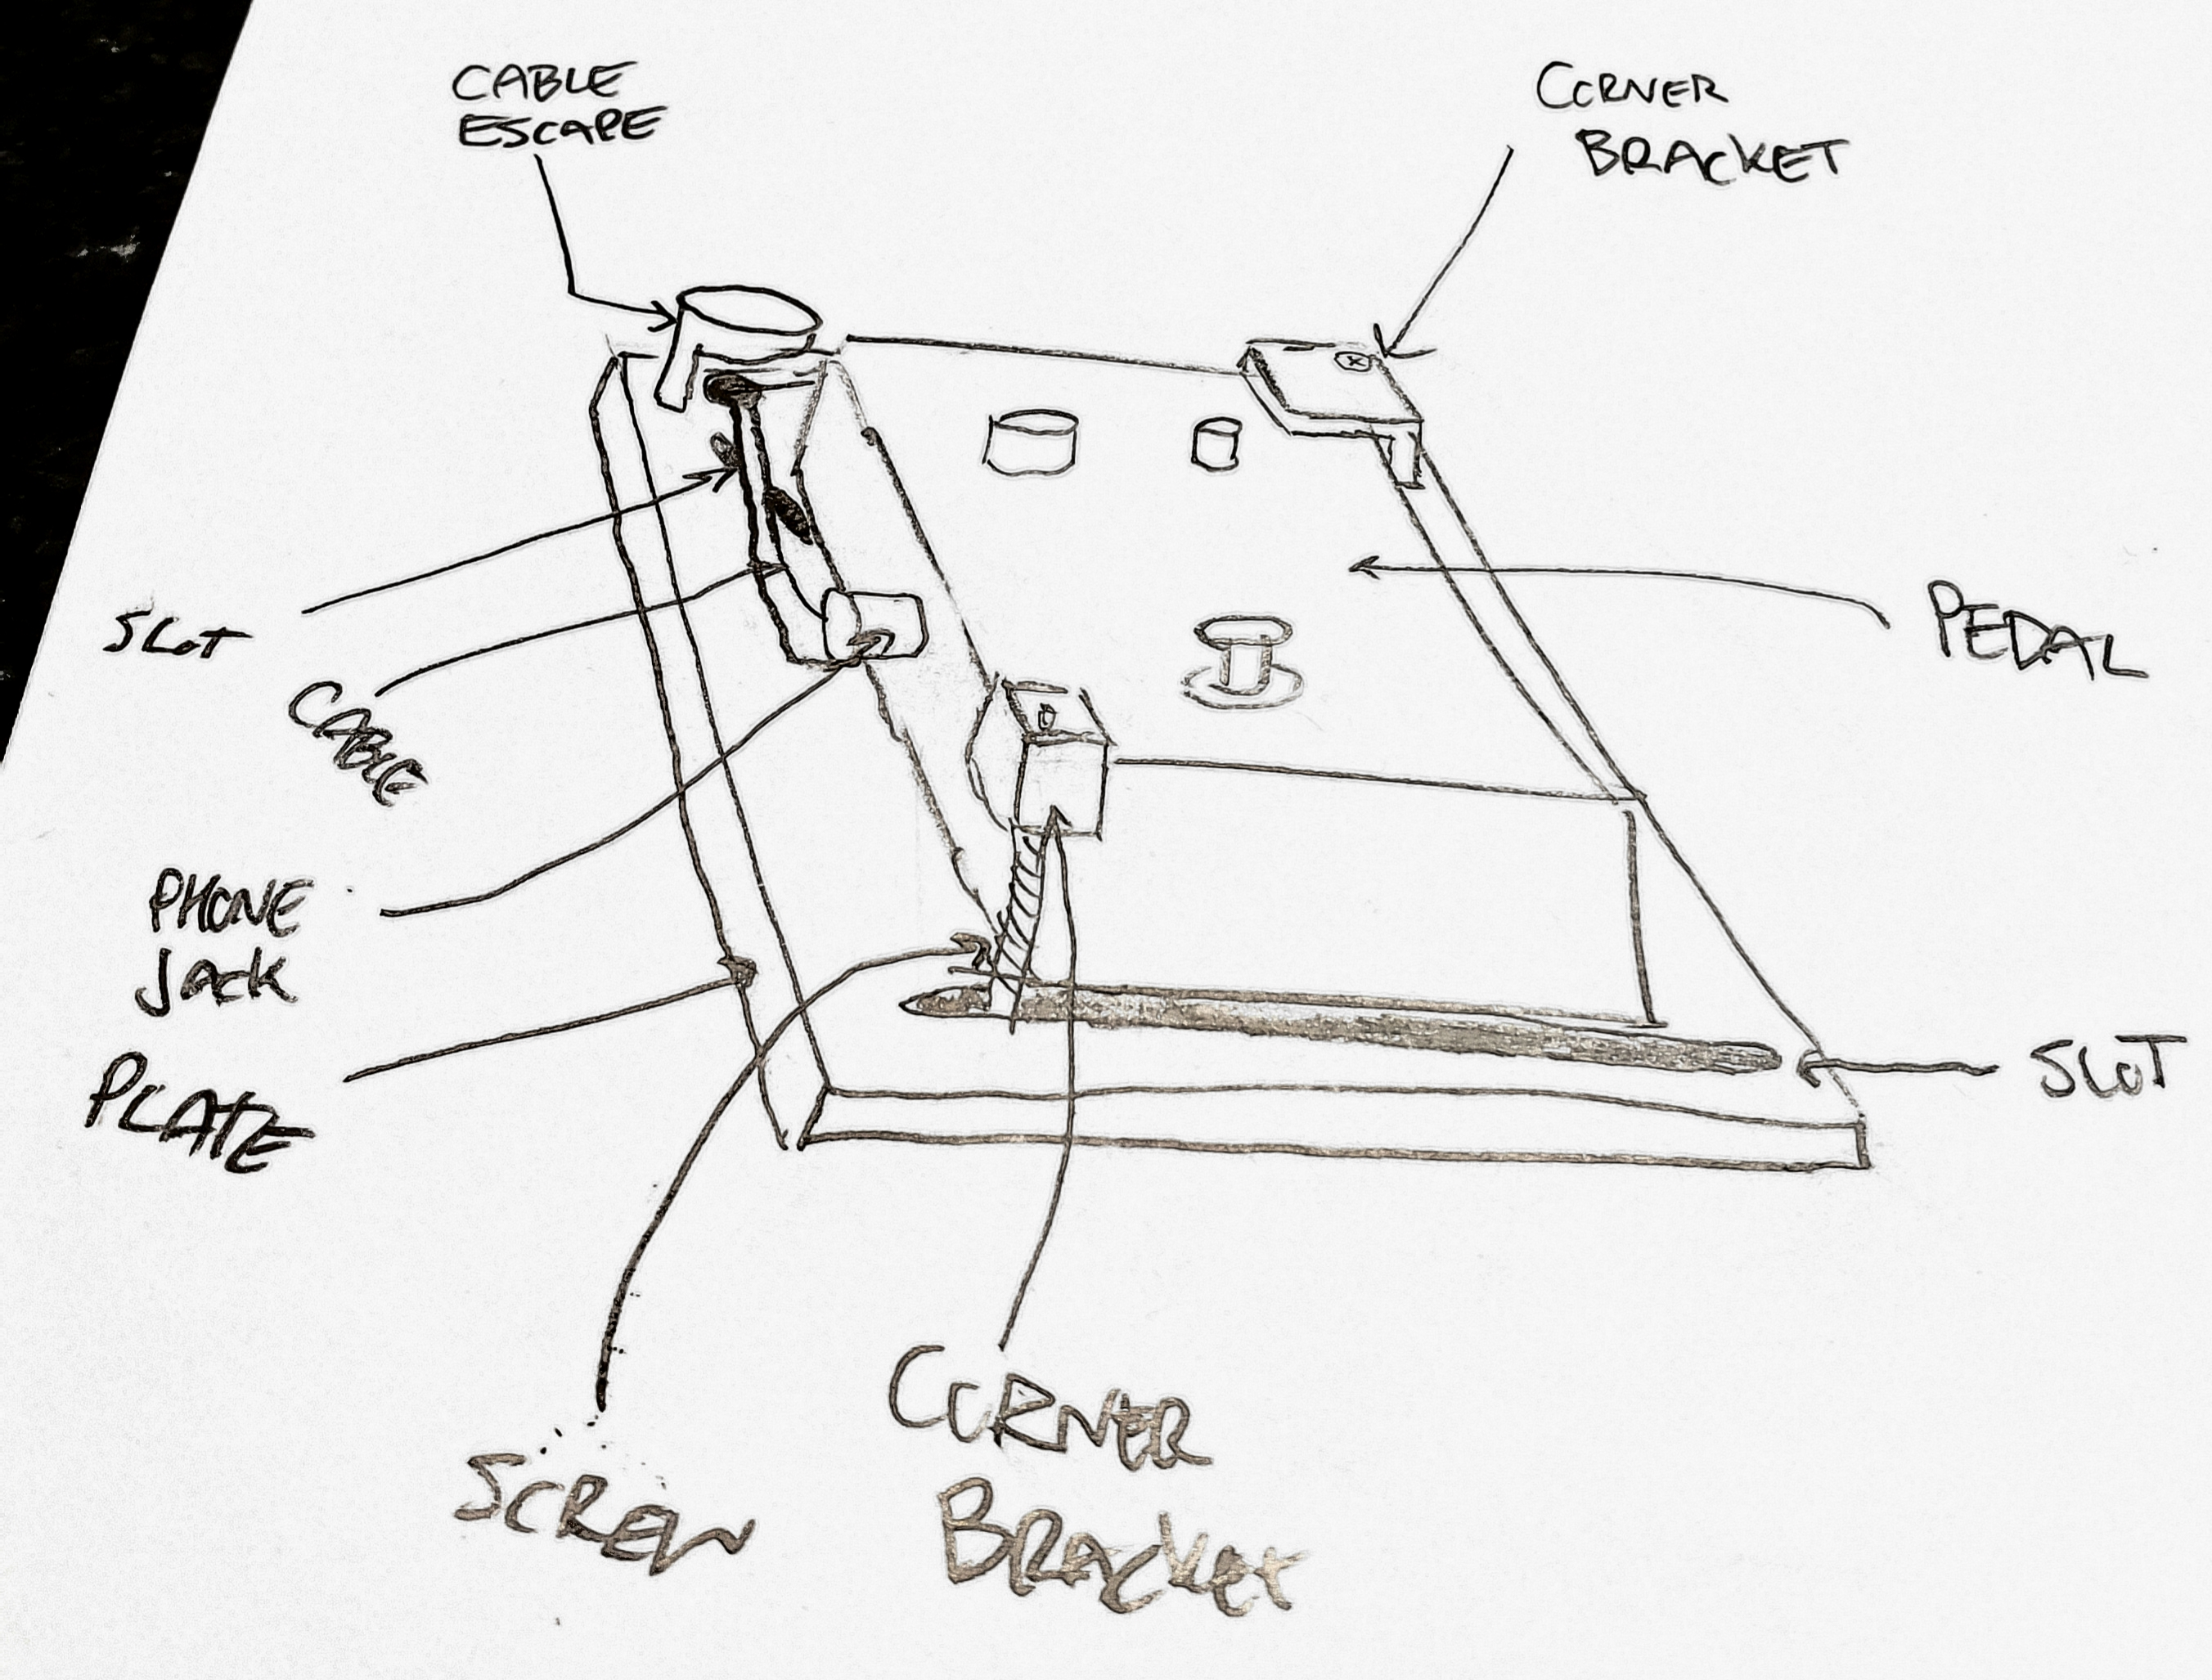
\includegraphics[width = 0.8 \textwidth]{PedalPlateSubsystemPerspective.jpg}
			\caption{Diagram of the interface between a guitar pedal and associated plate.  Note the corner brackets used as the mechanical attachment mechanism (bottom plate screws would have been hard to illustrate).  The cables escape from the plate via raised turrets.  Also note the slot just under the pedal where the bolt can move to accommodate pedals of different sizes.}
			\label{fig:PedalPlateSubsystem}
		\end{figure}

\section{Technical Specification}
	Note: see Analysis section for justifications
	\subsection{Size}
	\begin{itemize}
		\item Plate area should not exceed 10\% greater than the area of the largest pedal it supports
		\item Total floorspace should not exceed $ \approx 1 m^2$
		\item At least 8 pedal slots
	\end{itemize}
	% \begin{itemize}
	% 	\item To minimize wasted space, the area of each plate should not exceed 10\% more than the area of the largest effect pedal it supports.
	% 	\item The floorspace occupied by the entire device should not exceed $1m^2$, similar in size to current test setups.
	% 	\item The entire device should support at least 8 effects pedal slots.
	% \end{itemize}

	\subsection{Universality}
	Compatibility with $>$ 90\% $\pm 5\%$ of most popular effects

	\subsection{Pull Strength}
	Pull Force required to detach plate from board on the order of 30 Newtons $\pm 50\%$
	% The plates should be magnetically held to the board securely, yet with not too much force so they can still be easily removed.  The force required to lift the plates should be on the order of 25 - 50 Newtons.

	\subsection{Signal Characteristics}
		\begin{itemize}
			\item Bandwidth 2 Hz - 22 kHz
			\item Dynamic Range $>$ 96 dBV $+ 10\%, - 5\%$
		\end{itemize}

	\subsection{Reordering Time}
	10x improvement in swap time



\section{Preliminary Findings}
	\subsection{Size}
	To inform the design of the plates, I collected data on the physical dimensions of guitar pedals readily available at a Guitar Center retail location located on Boylston St. in Fenway.  I also collected data on which pedals were available in stock.  Typical dimensions were $2.5" \times 4.5"$, though there can be significant variation in size \cite{MyPedalData}.

	\subsection{Universality}
	In addition to the in-store data on in-stock pedals, I am also in the process of compiling data from major online sales venues, including Guitar Center.  Reverb, a major seller and reseller, provides some statistics on their sales for the past two years \cite{ReverbMostPopular}.  The most popular companies noted in these reports (namely Boss, Electro Harmonix, TC Electronic, and MXR) were also the most stocked brands at Guitar Center \cite{MyPedalData}.

	\subsection{Signal Characteristics}
	My thesis advisor Jim MacAurthur measured a signal to noise ratio on a generic electric guitar with humbucker pickups utilizing an Audio Precision instrument at 90dBV, by comparing the RMS voltage of the maximum output signal when the strings are struck hard ($\approx 1V_{RMS}$) to the RMS noise when the strings are muted.



\section{Analysis}

	\subsection{Size}
	Because of this project's shift in focus from a portable option for gigging guitarists, there is less constraint on the dimensions and portability of the unit.  This also means that it is acceptable for the user to leave slots unused.  However, the device should not be larger than typical display units, typically on the order of one square meter, which informed this specification.  To support a reasonable number of options for pedal combinations and routings, the board should accommodate at least four series effects, with at least two parallel chains.  This makes $2 \times 4 = 8$ pedal slots.

	\subsection{Universality}

	The data collected on the size of individual pedals shows general but not universal standardization in effects pedal size.  Though a given company typically offers their effects in at most three different sizes of enclosures, there is no standard between companies.  Although the most popular companies make up the majority of the market, this still leaves at least a dozen different form factors that a universal mounting plate should accept.  This will inform the design decision I will make in regards to the layout and attachment method of the plates.

	The design of the plate should strike a compromise between being general to as many products as possible while still being effective.  Both the "screw in" method \cite{ABBATE:2016} and a corner clamping method will be tested and evaluated on the first prototype.  Evaluations will be based on simplicity of attachment and resistance to dislodging due to shocks.  In addition to these methods of attaching the pedal to the plate, a number of plate layouts will be tested.  Prior to the first prototype several orientations of holes and slots for the screws to fit in will be examined and the most promising in terms of flexibility to accepting pedals of different sizes will be chosen to be included on the prototype.

	In addition to mechanical design, the project should support some pedals with different power requirements than the standard 9VDC.  While just 9VDC support would like cover the goal for 90\% of pedals, support for effects with 12VDC or 18VDC supplies would ensure near-universal compatibility.

	\subsection{Pull Strength}
	The force required to prise the pedal-plate from the its receptacle in the board must be both too strong to remove accidentally while light enough that a user can easily do so with one hand.  This will require testing of several strengths, and is one of the tests that will be conducted on the first prototype.

	\subsection{Signal Characteristics}
	The initial value expected for the signal to noise ratio for an electric guitar was near 120dBV.  Guitar pickups convert the mechanical energy of the vibrating strings to electrical energy via a coil of wire.  When the string vibrates in the magnetic field of a permanent magnet situated underneath, current is induced in the coil.  In an ideal environment, there should be little source of self noise because of the passive simplicity of this device, so any noise in the guitar signal is a result of the environment.  As such, the signal to noise ratio of a guitar can vary significantly based on the guitar's environment.  For example, guitar pickups are well known for their susceptibility to 60Hz line noise.  Therefore, the measured 90dBV signal to noise ratio should be taken as a minimum value, with 100dBV or more preferable.

	This will inform the design decision relating to the choice of switching element to use for implementing the routing and hot-swappable features.  While solid state switches are more size, cost, and power efficient than mechanical relays, they may not have adequate signal to noise specifications, as well as crosstalk between channels on the same chip.  For example, Microsemi/Zarlink's MT8808 Analog Switch Array mentioned in the project proposal \cite{Zarlink:MT8808} lists no specification on the device's signal to noise ratio, though it does boast a reasonable -90dB crosstalk between any channels for a 10kHz input with a $600 \Omega$ load.  The feed-through when a channel is off is listed as -95dB though, which is does not far exceed the minimum measured value for guitar signal to noise ratio, which could be an issue.  On the other hand, relay bypassing utilizing mechanical switches has no issues with signal to noise ratio, which would make it suitable for use in this project.

	As a minimum, the system should accommodate signals across the full range of human hearing, which is typically noted as 20Hz - 20kHz.  While this is the minimum acceptable range, there should also be allowance for lower and higher frequencies, which when used as input to a distortion effect can create inter-modulation distortion with frequencies in the audio range.  Neither of these ranges will be an issue however.  In the case that switching is accomplished with a solid state device, these are designed for frequency responses up to the tens of MHz range (the MT8808 has a 3dB frequency response of 45MHz), which is far greater than required.  If mechanical relays are used, there will likewise be no issues with frequency response in the audio range.  This specification will not inform the choice of switching element, but may come into play when designing any electronic buffers, amplifiers, or filters that may be required.

	In addition to these two considerations, there is also a bias among guitarists against solid state switching devices.  As previously mentioned, some implementations of electronic switching for guitar effects can result in signal degradation.  Though this presents an experimental reason for this bias, much of it can likely be attributed to guitarists' typical preference for "old school" approaches to their equipment.  For example, many guitarists still use vacuum tube amplifiers and analog distortion circuits to generate their sound rather than more modern techniques like digital signal processing.  This bias is likely more prevalent among users of this system; the most discerning customers will be most interested in choosing the best pedal for them, and may not "trust" the authenticity of the comparison if the test includes unnecessary circuit elements.  This bias, in addition to concerns over the signal to noise ratio of solid state switching elements has resulted in a preference to use relay switching technology for this project.

	\subsection{Reordering Time}
	This is the main metric to measure the success of this product in achieving its main aim of reducing the time required for a guitar is to test new guitar effects in different orders.  The most important test applied to both the current procedure and my prototypes and final product will be switching the order of two pedals.  This will both cover the time required to change out a single effect in the case of testing new products, as well as the case of switching effect routings.  The standard method of unplugging cables takes on the order of ten seconds, and the goal for this project is to reduce that time to on the order of one second, a 10x improvement.  The test must be conducted by a guitarist wearing a guitar, as this is how most users will interact with the product.  The test will also be done with different types of pedals to account for differences in size and shape, which could affect the required time.

	This measured time should not take into account the time required to set up a pedal for use with this system.  As the product will be designed for use as a sales tool in retail stores, the store employees will set up all applicable pedals in stock to be used with the system beforehand, so customers will only interact with the pedals integrated with their mounting plates.  Only when a customer decides to purchase a particular pedal and no other duplicate is in stock will the employee remove the pedal from the plate, which will be reused.  Though the time required to mount and dismount the pedal to the plates will not be accounted for in the swap time specification, it too must be measured and taken into account.  However, as there is little precedent for this, the specific specification may be difficult to precisely identify.  Instead, it must qualitatively be "unobtrusive": perhaps no longer than one minute per pedal.

\section{Updated Schedule}

The schedule has so far been working out, but though I am not behind on it yet, The schedule is fairly aggressive.  As I continue to get a better idea of the phases his project will go through, I will continue to both fill in the details for items as they approach and adjust the longer term goals accordingly.  The schedule for this semester has thus been updated, and will continue to be refined as I go.

Note: \colorbox{green}{Green text} indicates complete work.  \colorbox{yellow}{Yellow text} indicates work in progress.  \colorbox{red}{Red text} indicates items that are behind schedule.

\begin{table}[H]
\begin{tabular}{llp{4in}}
Weeks    & Dates         & Plan \\
\hline
1 \& 2   & 9/2 - 9/15    &  \colorbox{green}{Complete and revise Project Proposal and meet with advisers}      \\
3 \& 4   & 9/16 - 9/29   &  \colorbox{yellow}{Conduct experiments described above to help refine specifications.}  \colorbox{green}{Begin higher level block diagrams of system.  Progress Report \#1 due 9/28}    \\
5 \& 6   & 9/30 - 10/13  &  Begin prototyping key features, such as pedalboard - plate interface. Rapid prototyping of features such as plate design to inform first prototype. Develop lower level block diagrams and begin schematic design.    \\
7 \& 8   & 10/14 - 10/27 &  Electronic and Mechanical CAD design for first prototype.  The first prototype will be a single slot for testing the 1) reliability of electrical connections between plate and board, 2) mechanisms for attaching pedal to plate (mechanical and electrical), 3) strength of magnets needed to hold plate to board, 4) method for hot-swappable bypassing (sensing and actuation)    \\
9 \& 10  & 10/28 - 11/10 &  Test Prototype \#1.  Analyze results and make design decisions.  Refine design of routing mechanisms Progress Report \#2 due 11/5    \\
11 \& 12 & 11/11 - 11/24 &  Schematic entry, PCB design, and CAD modeling for refined Prototype \#2.     \\
13 \& 14 & 11/25 - 12/8  &  Fabricate mechanical parts.  Assemble circuit boards.  Perform preliminary testing on Prototype \#2 and begin iterating.      \\
15 \& 16 & 12/9 - 12/22  &  Summarize testing and outline goals/changes for next iteration.  Oral Design Review/Presentation 12/10    \\
17 \& 18 & 12/23 - 1/5   &  Winter Break: expect little progress    \\
19 \& 20 & 1/6 - 1/19    &  Work on firmware necessary for controlling routing and on-off switching for hot-swappability (may be done off-campus)    \\
21 \& 22 & 1/20 - 2/2    &  Complete firmware, iterate design if specifications are not met   \\
23 \& 24 & 2/3 - 2/16    &  Fabricate/Assemble iterated design and analyze.  Progress Report \#3 due 2/15    \\
25 \& 26 & 2/17 - 3/2    &  Analyze iterated design.    \\
27 \& 28 & 3/3 - 3/16    &  Implement reach features if time permits, else continue iterating and analyzing.  Begin outlines for Final Report.  Progress Report \#4 due 3/5   \\
28 \& 29 & 3/17 - 3/30   &  Prepare for presentation.  Write final report, make last minute changes.  Final Oral Presentation 3/25  \\
30 \& 31 & 3/31 - 4/13   &  Revise final report.  Final Written Report due 4/5    
\end{tabular}
\end{table}

\section{Updated Budget}

Like the schedule, the budget is becoming more clear than the one from the project proposal.  One piece of feedback I received from a number of people is the lack of representation in my budget for acquiring guitar pedals for testing and design purposes.  Some possible sources of pedals might be from my own personal collection, from a collection held by the Music Department, and by interested Harvard affiliates and professors.  Purchasing pedals for this project seems to be an unnecessary expense, so I will avoid purchasing new units if possible.  The budget for electronics and mechanical components might look like:

\begin{table}[H]
\begin{tabular}{llll}
Item                     & Quantity & Unit Cost & Total      \\
\hline
2 layer PCB from PCBgogo                    & 2        & $\sim$\$60 (depends on size) & $\sim$\$120     \\
Phone Connectors Mono Male (CUI)            & $\sim$18     & \$3.50    & $\sim$\$60 \\
NRJ6HM1 Phone Connectors Female (Neutrik)   & $\sim$4      & \$0.60    & $\sim$\$2  \\
Low Signal Relays - PCB DPDT NL 5VDC		& $\sim$42& \$1.55	  & \$65 			\\
Misc Electronic Components                  &         &           & \$30 ?          \\
Microcontroller                             & 1       & $\sim$\$5 & \$5             \\
4 lbs pull neodymium magnets, McMaster      & 2 x 8   & \$5       & \$80            \\
Misc mechanical components, materials       &         &           & \$100           \\
\textbf{Total}                              &         &           &  $\sim$\$460    \\
\end{tabular}
\end{table}

Most of the major components such as the relays and jacks can be reused between prototypes, as they are not very delicate or heat sensitive.  This will save cost between prototype iterations.  Getting PCBs manufactured is relatively expensive, so effort will be made to attempt fabricating simple PCBs with the PCB milling machine in the Active Learning Labs.

\section{Other Notes}

	\subsection{Glossary}
	Because this is a fairly unique product, accurately and precisely describing it will require a set of consistent definitions.  Though there was no time to develop such a system for this first progress report, this is one of the tasks listed on the updated schedule.  

	\subsection{Limiting Scope by Company}
	As described, developing a general design to universally fit pedals from all manufacturers is difficult because of lack of standardization between companies.  However, if the product was targeted towards a particular company, then integration with their products could be made much neater, as no company offers effects in more than a handful of form factors.  Though this might improve the effectiveness of the product, it may limit the scope too much.


\newpage
\bibliographystyle{plain}
\bibliography{ThesisSources}


\end{document}
